\documentclass[11pt]{article}
\usepackage{amsmath,amsfonts,amssymb,amsthm,fullpage,graphicx}
\DeclareMathOperator{\Dirichlet}{Dirichlet}
\title{SPARC Probability Materials}
\newtheorem{theorem}{Theorem}[section]
\newtheorem{lemma}[theorem]{Lemma}
\newtheorem{proposition}[theorem]{Proposition}
\newtheorem{corollary}[theorem]{Corollary}

\newenvironment{definition}[1][Definition]{\begin{trivlist}
\item[\hskip \labelsep {\bfseries #1}]}{\end{trivlist}}
\newenvironment{example}[1][Example]{\begin{trivlist}
\item[\hskip \labelsep {\bfseries #1}]}{\end{trivlist}}
\newenvironment{remark}[1][Remark]{\begin{trivlist}
\item[\hskip \labelsep {\bfseries #1}]}{\end{trivlist}}

\newenvironment{solution}[1][Solution]{\begin{trivlist}
\item[\hskip \labelsep {\bfseries #1}]}{\end{trivlist}}

\DeclareMathOperator{\Var}{Var}

\begin{document}
\maketitle

Random SPARC-related thought: there are typically NSF grants for high school outreach programs. If we wanted SPARC to remain free in future years, it might be good to look into these. Also companies such as Google, and probably other companies that I'm not thinking of right now.

\section{Probability and Expected Value}
\subsection{Probability: Formalizing ``Likeliness''}

It is 1954 (QQQ check year QQQ) and the government is holding a draft for soldiers to fight in World War II. You want to plan for the eventuality of being drafted, but in order to do this, you want to know how likely you are to actually be drafted.

You are planning a vacation to Hawaii, but are worried about being caught by a hurricane while visiting. How likely is this to occur for any given one-week period?

[marginalization example] If two six-sided dice are rolled, what is the probability that their sum is at least $8$? (QQQ okay this one is kind of lame... QQQ)


Your friend flips a coin ten times and it comes up head all ten times. How much evidence is this that the coin is rigged? What if it came up heads 8 times and tails twice?

[cancer test]

[Monte Hall]

In all of these situations, we are interested in how likely something is to occur; usually the answer to this is important for our future planning and decision-making. But, as you can see, one quickly runs into complex situations where intuition alone is unlikely to yield the best answer. This motivates the need for a formalization of the notion of likeliness. It is this notion of likeliness that we refer to as \textbf{probability}.

A formal mathematical treatment of the notion of probability is neither necessary nor possible (given time constraints) to give in this lecture. However, it is good to have some agreed-upon definition, so let us start by proposing the following:

\begin{definition} The probability of X is the fraction of outcomes (from a set of possible alternatives) with property X. \end{definition}

Is this a good definition of probability? What about the following question: \emph{A weighted coin comes up heads $10.2 \%$ of the time. If it is flipped twice, what is the probability that both results will be heads?} The issue is that while there are four alternatives (TT, TH, HT, HH), they are not all equally likely. We will therefore expand our definition to include alternatives with different degrees of likeliness.

\begin{definition} The probability of X is the total \emph{weighted} fraction of outcomes (from a set of possible alternatives) with property X. \end{definition}

As hinted at above, we can better formalize this using notions from calculus, functional analysis, and measure theory, but that is beyond the scope of this lecture (ask one of the instructors afterwards if you're interested).

(QQQ Actually, I'm still really confused as to how to empirically formulate the notion of probability, since it seems to inherently deal with counterfactuals...maybe someone else has a better idea? QQQ)

Our formalization is pointless unless we can solve problems with it, so let's go over how to solve a few of the problems given above.

\begin{example}
It is World War II, and you want to know how likely you are to be drafted.

What is the set of alternatives in this problem? We could look at the set of all possible drafts, and see how many have the property that we end up getting drafted. If there are $N$ draft-eligible people in the U.S., and $K$ get drafted, then there are $\binom{N}{K}$ possible drafts. How many of these involve you getting drafted? Given that you are drafted, there are $K-1$ additional people to be drafted among the $N-1$ remaining people, so there are $\binom{N-1}{K-1}$ possible drafts where you get drafted. The probability of you getting drafted is therefore $\frac{\binom{N-1}{K-1}}{\binom{N}{K}} = \frac{K}{N}$.

Alternately, we could consider the set of alternatives to be the set of draft-eligible citizens, and consider the probability that a citizen is drafted. Then $K$ of the $N$ citizens are drafted, so the probability is again $\frac{K}{N}$. Since all citizens are presumably indistinguishable from the perspective of the draft, we should treat ourselves as a generic citizen, and therefore the probability is again $\frac{K}{N}$.
\end{example}

\begin{example}
What is the probability that Hawaii gets hit by a hurricane during a given one-week period?


\end{example}

\subsection{Marginalization and Hidden Variables}

We will now introduce another tool into our toolkit, called \emph{marginalization}, which is motivated by the third example above.

\subsection{Conditioning and Observed Variables}
\subsection{Combining Events: Independence and Boolean Logic}
\subsection{Expected Value}
\subsection{Problems}
\begin{enumerate}
\item Two six-sided dice are rolled. What is the probability that the first die lands on either $2$, $3$, or $4$, and that the second lands on either $1$ or $5$?
\item Show that $\frac{p(x \mid y)}{p(y \mid x)} = \frac{p(x)}{p(y)}$.
\item (von Neumann's trick) Suppose that a coin comes up heads with some unknown probability $p$. Show how, by flipping the coin twice, we can simulate a coin that comes up heads with probability $\frac{1}{2}$. (Hint: in some cases it will be necessary to re-do the two flips.)
\item (Monty Hall problem) Suppose you're on a game show, and you're given the choice of three doors: Behind one door is a car; behind the others, goats. You pick a door, say number 1 [but the door is not opened], and the host, who knows what's behind the doors, opens another door, say number 3, which has a goat. He then says to you, ``Do you want to pick door number 2 instead?'' Is it to your advantage to switch your choice? What is the probability of getting the car if you do switch your choice?
\item Consider the following simple evolutionary model: at each time $t$, there are $N$ organisms, each of which has a single gene equal to either type $A$ or type $B$. Between time $t$ and time $t+1$, each organism splits into two copies (with the same genotype as the original), and then half of the organisms die at random, so that the population remains at $N$.
\begin{itemize}
\item[a.] Show that, eventually, either all organisms will be type $A$ or type $B$ (this is called \emph{fixation}).
\item[b.] Initially, there are $k$ organisms of type $A$ and $N-k$ of type $B$. What is the probability that all organisms end up as type $A$?
\item[*c.] Approximately how long will it take for fixation to occur, as a function of $N$ and $k$? (You can neglect constant factors.) (QQQ This should be something like $\log(k)+\log(N-k)-\log(N)$, but we should probably double-check that it's at least solvable in principal. I had to use Markov's inequality. QQQ)
\end{itemize}
\item Start with a uniform distribution over a sphere. What is the conditional distribution given that the latitude is zero (i.e. conditioning on lying on the equator)? What about the conditional distribution given that the longitude is zero (i.e. conditioning on lying on a circle going through both poles)? Are they the same or different?
\item A set of probability distributions $p_1,p_2,\ldots$ is \emph{consistent} if the variables in $p_k$ are a subset of the variables in $p_{k+1}$ and the marginal distribution of $p_{k+1}$ is $p_k$. It is \emph{exchangeable} if re-ordering the variables doesn't change the distribution.
\begin{itemize}
\item Let $p_k$ be a distribution over the results of $k$ coin flips. Show that drawing the coin weight from a uniform distribution and then flipping the coins independently yields a consistent and exchangeable family of distributions.
\item * Let $p_k$ be a distribution over binary trees with nodes labelled $1,\ldots,k$. Can you define a consistent family of distributions $\{p_k\}_{k=1}^{\infty}$? You will probably have to slightly modify the notions of consistency and exchangeability given.
\end{itemize}
\end{enumerate}
\section{Bayesian Modeling}
\subsection{Subjective Probability}
``I think there's a 40\% chance that it will rain tomorrow.'' What do we mean when we make such a statement? Expressing \textbf{subjective uncertainty} is one of the most useful applications of the formalism of probability theory, and forms the foundation for a large subset of statistical machine learning. As a simple example, let us return to the coin-flipping example of yesterday.

\begin{example}
A coin is flipped ten times and comes up heads eight out of the ten times. How likely is the coin to be rigged?
\end{example}

\begin{solution}
A priori, most coins tend to be fair, so let us assign $90\%$ probability to the coin being fair and $10\%$ to it being rigged. If it is fair, then it comes up heads with probability $0.5$. If it is rigged, then it comes up heads with some unknown probability $w \in [0,1]$, over which we will place a uniform distribution.

Now we need to condition on the observed data. By Bayes' rule, 
\[ p(\mathrm{Fair} \mid \mathrm{H^8T^2}) \propto p(\mathrm{H^8T^2} \mid \mathrm{Fair}) \times p(\mathrm{Fair}) = 0.9 \times 0.5^10 \approx 8.79 \times 10^{-4}. \]
Again applying Bayes' rule, 
\[ p(\mathrm{Rigged} \mid \mathrm{H^8T^2}) \propto p(\mathrm{H^8T^2} \mid \mathrm{Rigged}) \times p(\mathrm{Rigged}) = \int_{0}^{1} w^8(1-w)^2 dw \times 0.1 = 2.02 \times 10^{-4}. \]
So, $p(\mathrm{Rigged} \mid \mathrm{H^8T^2}) = \frac{2.02}{2.02+8.79} = 0.19$. Therefore, the coin is not all that likely to be rigged. 
\end{solution}

The approach given in the solution is an example of a \textbf{probabilistic generative model}. It consists of a \textbf{prior} $p(\theta)$ over a collection $\theta$ of \textbf{latent parameters} (in this case, whether the coin was rigged, together with the parameter $w$) and a \textbf{likelihood} $p(X \mid \theta)$ over the observed data (the probability that a given set $X$ of data would be generated, conditioned on the latent parameters; in this case, the probability of a sequence of coin flips). In order to make new predictions based on our current data, we compute $p(\theta \mid X)$ and then use this to compute $p(X_{\mathrm{new}}) = \int p(\theta \mid X) p(X_{new} \mid \theta) d\theta$. So, in the end what we are doing is constructing classes of models that predict observations (parameterized by $\theta$), weighting the models based on how well their predictions match the actual observations we see, and then predicting future observations by looking at the predictions of each of our models based on how well they have done in the past.

(QQQ introduce the words \textbf{posterior}, \textbf{predictive}, and \textbf{inference}; for inference make sure to talk about the ambiguity in how it is used in practice in the ML community QQQ)

\subsection{Causal Reasoning}
Consider the following three situations:

\begin{itemize}
 \item If a colleague ignores you one day, do they dislike you or are they simply busy? What if they ignore you three days in a row?
 \item If an alarm goes off, is a burglary occurring? What if it is the middle of an earthquake?
 \item If a student does well on an exam, are they intelligent? What if everyone else did poorly on the exam?
\end{itemize}

We will now show how to use probabilistic reasoning to answer all three of these questions. In the first case, we can compute

\[ \frac{p(\mathrm{Busy} \mid \mathrm{Ignores})}{p(\mathrm{Dislikes} \mid \mathrm{Ignores})} = \frac{p(\mathrm{Ignores} \mid \mathrm{Busy})}{p(\mathrm{Ignores} \mid \mathrm{Dislikes})} \frac{p(\mathrm{Busy})}{p(\mathrm{Dislikes})}. \]

On the other hand, if we are ignored three days in a row, we are comparing the hypothesis that they are busy on three separate days to the hypothesis that they simply dislike us. Then the above equation becomes

\[ \frac{p(\mathrm{Busy} \mid \mathrm{Ignores})}{p(\mathrm{Dislikes} \mid \mathrm{Ignores})} = \frac{p(\mathrm{Ignores} \mid \mathrm{Busy})^3}{p(\mathrm{Ignores} \mid \mathrm{Dislikes})^3} \frac{p(\mathrm{Busy})^3}{p(\mathrm{Dislikes})}, \]

so it becomes less likely that the other person is busy and more likely that they dislike us (unless it is substantially more likely that they would ignore us when they are busy than when they dislike us).

In the second example, there are two rival explanations for the alarm going off --- a burglary and an earthquake. An earthquake is readily observable, and so if we don't see one then the cause of the alarm is probably a burglary. On the other hand, if we do see an earthquake, then that is probably why the alarm is going off, so we have no reason to suspect a burglary.

Make sure that you know how to formalize the above examples in terms of probabilities. \textbf{Hint:} You'll need to consider $p(\mathrm{Alarm} \mid \mathrm{Presence of earthquake, presence of burglary})$, and assume that it is higher both when there is an earthquake and a burglary.

Finally, in the third example, we can consider two rival causes for our observation that the student did well on the exam --- either the student is intelligent, or the exam is easy. If the exam is easy, then it is quite unlikely that all the other students would do poorly on it. Therefore, if all the other students do poorly, then the exam is probably not easy, so the student is probably intelligent.

Again, make sure that you know how to formalize the above example.

\subsection{Mixture Models}
We will now begin to consider more complicated models, where the posterior probabilities cannot necessarily be computed in closed form or by hand. We will later discuss computational methods for computing posterior distributions, but for now will ignore exact computations and focus on qualitative analysis of the models. In this section, we will look at a class of models based on the assumption that the likelihood for each data point is determined by one of a small collection of underlying latent features. Such models are called \textbf{mixture models}, because the predictive distribution is a discrete mixture of distributions based on each of the possible settings of the latent features.

\subsubsection{Testing Correlations}

Suppose that we have a sequence of pairs $(X_i,Y_i)$ of observations, where $i$ ranges from $1$ to $n$. For instance, $X_i$ could be the event that person $i$ is Hispanic, and $Y_i$ could be the event that person $i$ voted for Barack Obama in the 2008 election. A natural question to ask is whether $X_i$ and $Y_i$ are correlated with each other. How can we model this?

If $X_i$ and $Y_i$ are uncorrelated, then the joint probability $p(X_i,Y_i)$ can be given in terms of two parameters, $\theta := p(X_i = \mathrm{True})$ and $\phi := p(Y_i = \mathrm{True})$. (The ``$:=$'' symbol means ``is defined to be''.) Then the joint probability table is

\vskip 0.1in

\begin{tabular}{|c|c|c|}
\hline
 & $X_i = \mathrm{False}$ & $X_i = \mathrm{True}$ \\
\hline
$Y_i = \mathrm{False}$ & $(1-\theta)(1-\phi)$ & $\theta(1-\phi)$ \\
\hline 
$Y_i = \mathrm{True}$ & $(1-\theta)\phi$ & $\theta\phi$ \\
\hline
\end{tabular}

\vskip 0.1in

If we let $X$ denote the indices where $X_i$ is true, and $Y$ denote the indices where $Y_i$ is true, then $p(\{X_i,Y_i\}_{i=1}^n \mid \mathrm{Uncorrelated}) = \frac{|X|!|X^C|!|Y|!|Y^C|!}{(n+1)!^2}$, where $S^C$ is the complement of $S$. Note that this computation as well as the rest in this section involves taking potentially complicated integrals. I'm skipping over them because I think going through the calculations would detract from the exposition.

Now, how do we model correlated data? We could just pick variables for the four entries of the above joint probability table, and then constrain their sum to be $1$. This would give us $p(\{X_i,Y_i\}_{i=1}^n \mid \mathrm{Correlated}) = \frac{|X \cup Y|!|X \cup Y^C|! |X^C \cup Y|! |X^C \cup Y^C|!}{(2n+3)!}$. (QQQ check this computation QQQ)

I think a more interesting model that might more accurately capture the intuitive causal structure is to assume that each person belongs to one of two groups, the first with characteristics $\theta_1$, $\phi_1$, and the second with characteristics $\theta_2$, $\phi_2$.

This allows correlations as follows --- Suppose that $\theta_1$ and $\phi_1$ are both high, and $\theta_2$ and $\phi_2$ are both low. Then whenever $X_i$ is true, person $i$ is likely to belong to group $1$, and therefore $Y_i$ is also likely to be true. Conversely, if $X_i$ is false, then person $i$ is likely to belong to group $2$, and therefore $Y_i$ is also likely to be false.

Note that in addition to $\theta_1$, $\phi_1$, $\theta_2$, and $\phi_2$, we need to specify a parameter $\pi$ which is the probability that someone belongs to group $1$. Then we get the following joint probability table:

\vskip 0.1in

\begin{tabular}{|c|c|c|}
\hline
 & $X_i = \mathrm{False}$ & $X_i = \mathrm{True}$ \\
\hline
$Y_i = \mathrm{False}$ & $\pi(1-\theta_1)(1-\phi_1)+(1-\pi)(1-\theta_2)(1-\phi_2)$ & $\pi\theta_1(1-\phi_1)+(1-\pi)\theta_2(1-\phi_2)$ \\
\hline 
$Y_i = \mathrm{True}$ & $\pi(1-\theta_1)\phi_1+(1-\pi)(1-\theta_2)\phi_2$ & $\pi\theta_1\phi_1+(1-\pi)\theta_2\phi_2$ \\
\hline
\end{tabular}

\vskip 0.1in

Unfortunately, it is not actually possible to evaluate the integral that would result from the above joint probability table in closed form. (QQQ insert further exposition here, and perhaps the results of MCMC QQQ)

Note that in the situation we gave, there are probably many more people whose ethnicity we know (due to the census) than people whose voting decision we know. Therefore, there are many $i$ for which we know $X_i$ but not $Y_i$. Can we incorporate this into our model? Yes! If we only know $X_i$, then $p(X_i = \mathrm{True} \mid \pi, \theta, \phi) = \pi\theta_1+(1-\pi)\theta_2$. Note that we can also easily make predictions such as the probability that someone voted for Barack Obama given that they are Hispanic. The ability to seamlessly deal with incomplete data or condition on partial information is one of the benefits of using probabilistic generative models.
\subsubsection{Binary Mixtures}

The above example leads us into a more general method of detecting correlations in data. It is helpful for making intuitive judgments about when possessing one collection of properties leads someone to possess an additional collection of properties. This is called a \textbf{binary mixture model}. Suppose that we have a sequence of $n$ observations, but this time each observation $X_i$ consists of $t$ binary data points, $X_{i,1}$, $X_{i,2}$, $\ldots$, $X_{i,t}$. We refer to these as \textbf{features}, and we will label them $F_1$ through $F_t$. If $X_{i,j}$ is true then we say that object $i$ possesses feature $j$. So, as before, the objects could be different people and the features could be characteristics of each of these people.

We would like to construct a model that allows us to make inferences like: ``How likely is an object to possess $F_k$ given that it possesses $F_j$?''

We can do this by assuming that each object comes from one of $k$ clusters, where cluster $i$ has parameters $\{\theta_{i,j}\}_{j=1}^t$, with $\theta_{i,j}$ specifying the probability that an object has feature $j$ if it is from cluster $i$. We also have probabilities $\pi_1,\ldots,\pi_k$, with $\pi_1+\pi_2+\ldots+\pi_k=1$, where $\pi_i$ specifies the probability that an object is drawn from cluster $i$.

Now if a set of features is correlated, our model can learn this by making one of the similarity clusters assign high probability to each of those features. If an object has some of those features then it probably comes from that cluster, and therefore probably has the rest of those features. (QQQ more concrete example QQQ)

\subsubsection{Gaussian Mixtures}

A more visually intuitive variant of the binary mixture model is the \textbf{Gaussian mixture model}. Suppose that we see the following set of points:

\begin{center}
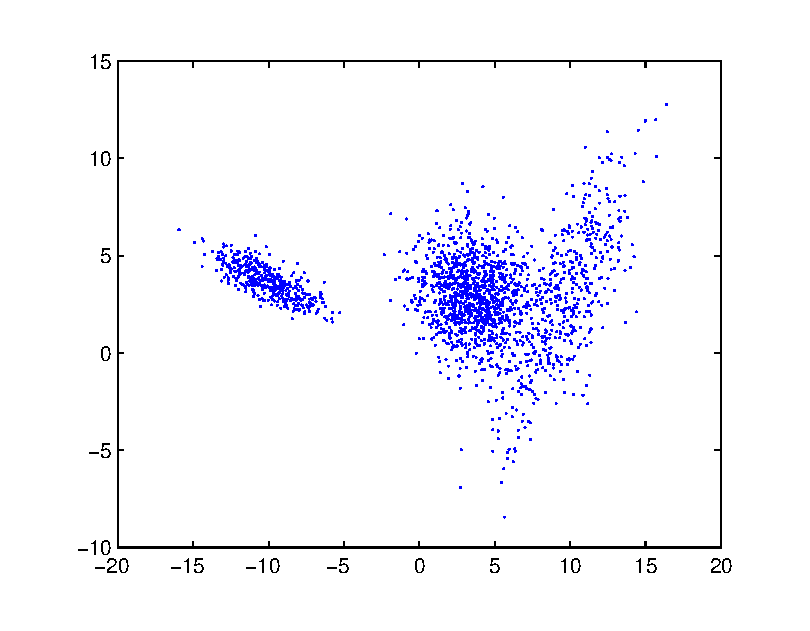
\includegraphics[width=0.4\textwidth]{mixture.eps}
\end{center}

It is pretty clear that the data is clustered, probably with three clusters. We can model this by saying that each data point is drawn from one of three Gaussian distributions (a Gaussian is the generalization of a bell curve to two dimensions and higher). Once we have this model, we can ask questions like the probability that a new point came from each of the three clusters, or the predictive distribution of its $y$-coordinate given its $x$-coordinate.

(QQQ show inference occurring QQQ)

\subsubsection{Missing Data and Partially Labelled Data}

(QQQ TODO QQQ)

\subsection{Hidden Markov Models}

We now come to one of the most famous examples of probabilistic modeling --- hidden Markov models (HMMs). These are often used when we have some process that evolves in time, and noisy observations about the state of that process.

The usual setup for an HMM is a sequence of points in time, indexed by the integers $1$ through $n$. We assume that there is some system that we care about, and that the state of that system at time step $i$ is $S_i$. We further assume that we can perform (imperfect) measurements of certain aspects of the system, and that the measurement at time $i$ is $M_i$. $S_i$ only depends on $S_{i-1}$, and $M_i$ depends only on $S_i$.

For instance, our system might be a point in two-dimensional space, and we might have noisy observations about the location of that point. If $S_i = \left[ \begin{array}{c} x_i \\ y_i \end{array} \right]$, let's suppose that we know that

\begin{eqnarray*}
x_{i+1} & = & 0.995 x_{i} - 0.05 y_{i} \\
y_{i+1} & = & 0.995 y_{i} + 0.05 x_{i}
\end{eqnarray*}

A typical trajectory for this system is

\begin{center}
 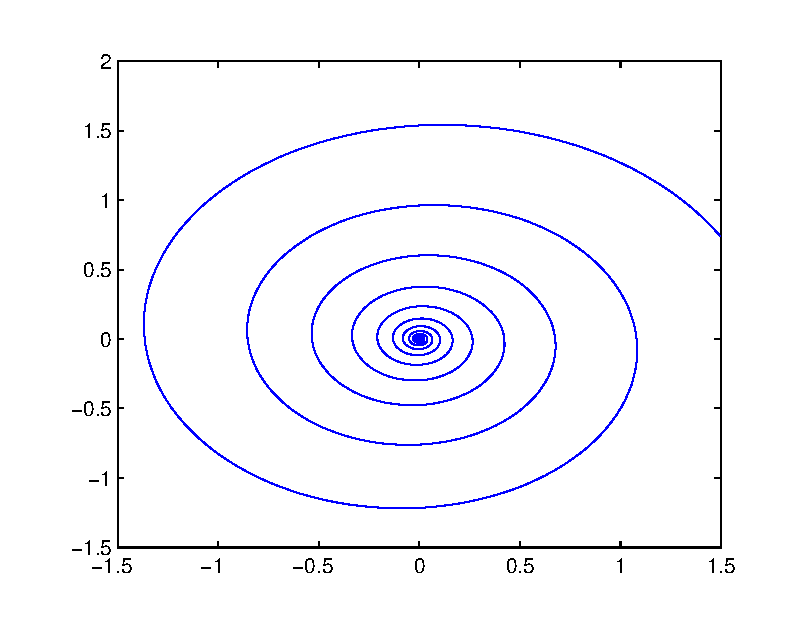
\includegraphics[width=0.6\textwidth]{traj1.eps}
\end{center}

Suppose that we can take measurements of the system that have Gaussian white noise with standard deviation $0.1$. Then a typical measurement history is

\begin{center}
 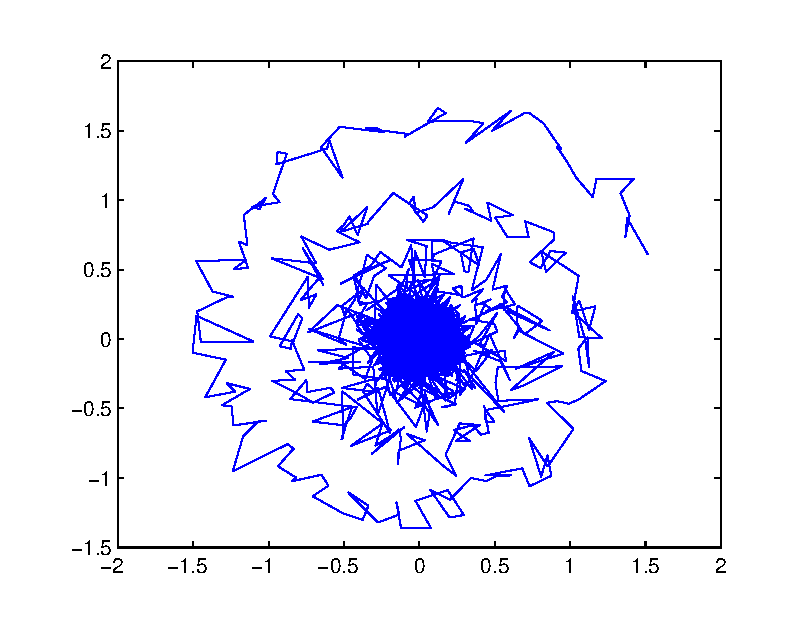
\includegraphics[width=0.6\textwidth]{traj2.eps}
\end{center}

and with white noise with standard deviation $1.0$ it is

\begin{center}
 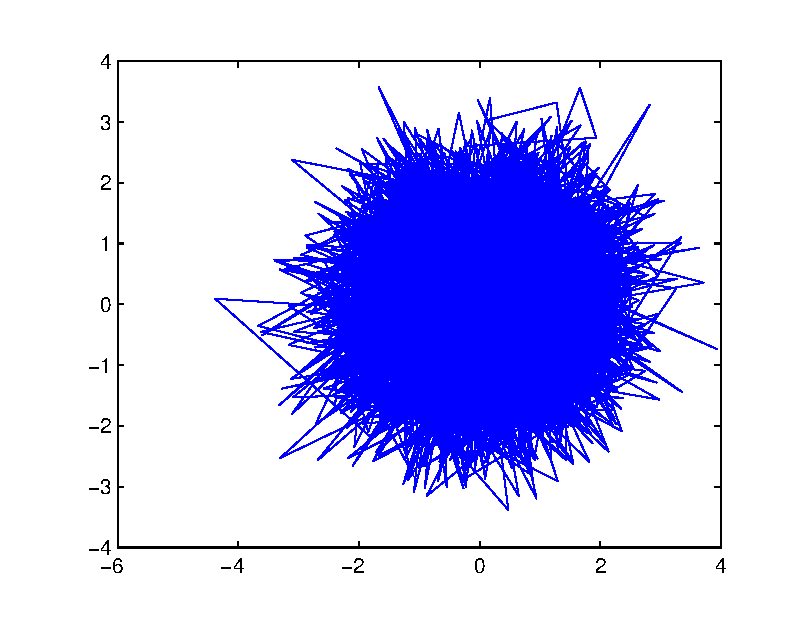
\includegraphics[width=0.6\textwidth]{traj3.eps}
\end{center}

The amazing thing is that, by performing inference on the HMM with $M_i = S_i + N_i$, where $N_i$ is the assumed Gaussian white noise, we can recover the evolution of the system even from extremely noisy histories as above. This is known as a \textbf{Kalman filter}. In the image below, the blue curve is the actual state history, and the red curve is the estimated history using a Kalman filter. Note that the high degree of noise means that it takes a fairly large number of estimates to converge on the correct trajectory.

\begin{center}
 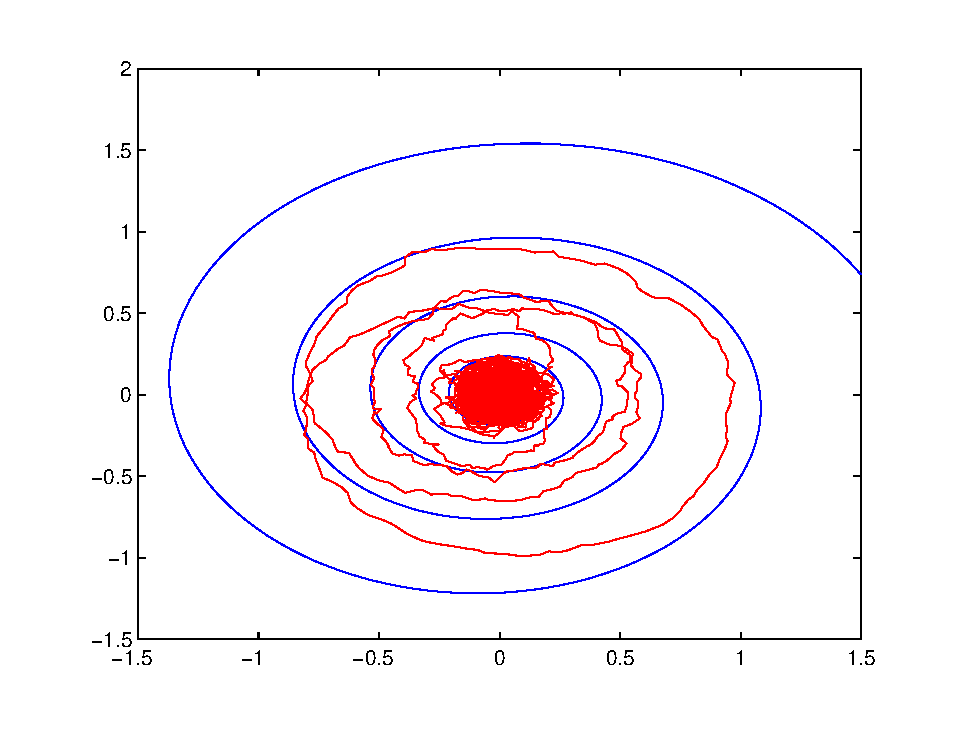
\includegraphics[width=0.6\textwidth]{traj4.eps}
\end{center}


\subsection{Components of Generative Models}

(QQQ go over stuff like beta, Dirichlet, Gaussian, normal-inverse Wishart, gamma, and exponential families QQQ)

\subsection{Probabilistic Inference}



\subsection{Problems}
\begin{enumerate}
\item You see a strange coin, where you suspect that either consecutive flips are independent, or else that the next flip is equal to the previous flip with some unknown probability $p$ (i.e., the coin has ``memory'').
\begin{itemize}
\item[a.] Build a simple Bayesian model for this situation. If you don't know calculus, you can assume that the coin weight / switching probability is always equal to either $\frac{1}{4}$, $\frac{1}{2}$, or $\frac{3}{4}$.
\item[b.] You observe the sequence HHHTTHHHTTTTHH. What is the probability that the coin has memory in the sense described above?
\item [c.] How sensitive is this probability to your priors? What if the sequence was only HHHT?
\end{itemize}
\item The \emph{Dirichlet distribution} is often used as a prior over an unknown probability distribution $\pi$. If $\pi$ is a distribution over $N$ outcomes, then we can treat $\pi$ as an $N$-dimensional vector $\pi_1,\ldots,\pi_N$ such that $\pi_i \geq 0$ and $\sum_{i=1}^{N} \pi_i = 1$. A Dirichlet distribution has non-negative parameters $\alpha_1,\ldots,\alpha_N$. The probability density is given by 
\[ p(\pi) \propto \pi_1^{\alpha_1-1}\pi_2^{\alpha_2-1}\cdots\pi_N^{\alpha_N-1}. \]
In this problem, we will investigate the properties of the Dirichlet distribution, such as the normalization constant.
\begin{itemize}
\item[a.] Suppose that we observe a single sample $x_1$ from $\pi$, and that the value of the sample is $1$. What is $p(\pi \mid x_1=1)$?
\item [b.] In general, show that if we observe an arbitrary sequence of samples $x_1,\ldots,x_k$ from $\pi$, the distribution $\pi \mid x_1,\ldots,x_k$ is still Dirichlet-distributed, and calculate the values of the new parameters in terms of $\alpha$ and $x$. Due to this property, we say that the Dirichlet distribution is a \emph{conjugate prior} to the multinomial distribution (i.e., the distribution where we just sample a single discrete outcome).
\item [c.] Let $\alpha = (\alpha_1,\ldots,\alpha_N)$ and let $e_i$ be the vector that is $1$ in the $i$th coordinate and zero elsewhere. Show that $\Dirichlet(\alpha)$ is a mixture of $\Dirichlet(\alpha+e_i)$ where $i$ ranges from $1$ to $N$. (Hint: what happens if we sample a distribution $\pi$ from $\Dirichlet(\alpha)$, then draw a sample from $\pi$ and condition on the outcome?)
\item [d.] Let $Z(\alpha)$ be the normalization constant for $\Dirichlet(\alpha)$. Building on the previous part, show that, in fact, 

\[ \Dirichlet(\alpha) = \sum_{i=1}^N \frac{Z(\alpha+e_i)}{Z(\alpha)} \Dirichlet(\alpha+e_i) \]
\item [e.] Compute $\frac{Z(\alpha+e_i)}{Z(\alpha)}$. (Hint: you should be able to reduce this to a single-variable integral.)
\item [f.] Using the fact that $Z(1,1,\ldots,1) = 1$, compute $Z(\alpha)$.
\end{itemize}
\end{enumerate}
\section{Statistics}
Statistics can be thought of as the analysis of random variables (usually in the context of the interaction of a large number of random variables). Today we will cover several important inequalities that can be used to bound the behavior of random variables and families of random variables.
\subsection{Markov's Inequality}
The simplest inequality, called \textbf{Markov's inequality}, is actually the foundation of most other statistical inequalities.
\begin{theorem}[Markov's inequality]
Let $X$ be a non-negative random variable with mean $\mu$. Then $\mathbb{P}[X \geq t] \leq \frac{\mu}{t}$.
\end{theorem}
This may seem like a very weak inequality, but by applying well-chosen coordinate transformations to $X$ we can get much stronger results.
\subsection{Method of Moments}
The moment inequalities are all corollaries of Markov's inequality.
\begin{theorem}[$p$th moment inequality]
Let $X$ be a real-valued random variable. Then $\mathbb{P}[|X| \geq t] \leq \frac{\mathbb{E}[|X|^p]}{t^p}$.
\end{theorem}
Of special importance is Chebyshev's inequality:
\begin{theorem}[Chebyshev's inequality]
Let $X$ be a real-valued random variable with mean $\mu$. Then $\mathbb{P}[|X-\mu| \geq t] \leq \frac{\mathbb{E}[(X-\mu)^2]}{t^2}$.
\end{theorem}
We call $\mathbb{E}[(X-\mu)^2]$ the \textbf{variance} of $X$, or $\Var[X]$. The reason that Chebyshev's inequality is particularly useful is because 2nd moments have many nice computational properties:
\begin{lemma}
If $\mu = \mathbb{E}[X]$, then $\mathbb{E}[(X-\mu)^2] = \mathbb{E}[X^2]-\mu^2$.
\end{lemma}
\begin{lemma}
If $X_1,\ldots,X_n$ are real-valued random variables, and $X_i$ and $X_j$ are independent for all $i \neq j$, then $\Var[X_1+\cdots+X_n] = \Var[X_1]+\cdots+\Var[X_n]$.
\end{lemma}
Similar results hold for higher moments, but require stronger independence assumptions (e.g. $4$th moments require any $4$ random variables to be independent). (QQQ check whether this holds for odd and non-integral moments QQQ)
\subsection{Sub-Gaussian Variables and the Chernoff Bound}
In addition to moments, a very important statistical function is the \textbf{cumulant function}. 
\subsection{Law of Large Numbers and Central Limit Theorem}
\subsection{The Union Bound}
\subsection{Problems}
\begin{enumerate}
\item Doob's theorem for $[0,1]$ variables
\item Azuma-Hoeffding
\item de Finetti's theorem
\end{enumerate}
\end{document}